\section{Geometric Representation of \texorpdfstring{$\sqrt{2}$}{sqrt(2)} in Binary}
\subsection{Visual Overview}
The provided diagram illustrates the key mathematical properties of the binary expansion of $\sqrt{2}$ using geometric constructs:

\begin{itemize}
    \item \textbf{Outer Square and Red Diagonal:}
    \begin{itemize}
        \item The black square represents a unit square with a side length of 1.
        \item The red diagonal represents $\sqrt{2}$, the hypotenuse of this square. Its infinite binary expansion reflects its irrational nature, as no finite binary sequence can fully capture its value.
    \end{itemize}
    \item \textbf{Binary Approximation Process:}
    \begin{itemize}
        \item Successive blue dashed squares refine the approximation of $\sqrt{2}$ in binary. Each step represents a higher-order term in the binary series of $\sqrt{2}$, such as:
        $$\sqrt{2} = 1.0110101000001001111\ldots_2.$$
        \item Each binary digit corresponds to a geometric refinement, halving the remaining area of interest. For example:
        \begin{itemize}
            \item The first approximation, $1.1_2 = 1.5$, overestimates $\sqrt{2}$.
            \item The second refinement, $1.01_2 = 1.25$, brings the approximation closer, halving the error.
            \item The third refinement, $1.001_2 = 1.125$, further reduces the uncertainty by halving it again.
        \end{itemize}
    \end{itemize}
    \item \textbf{Green Circle: Irrational Gap Constraint:}
    \begin{itemize}
        \item The green circle illustrates the minimum gap between $\sqrt{2}$ and any rational approximation $\frac{p}{2^n}$. This gap is given by:
        $$\left|\sqrt{2} - \frac{p}{2^n}\right| \geq \frac{1}{2^{2n}},$$
        ensuring that the exact value of $\sqrt{2}$ cannot be represented with finite binary digits.
    \end{itemize}
    \item \textbf{Zero Run Bounds:}
    \begin{itemize}
        \item Runs of zeros in the binary expansion correspond geometrically to periods where successive approximations maintain their positions relative to $\sqrt{2}$. These zero runs are limited by the logarithmic bound:
        $$k \leq \log_2(n),$$
        where $k$ is the zero run length at position $n$.
    \end{itemize}
\end{itemize}

\begin{center}
    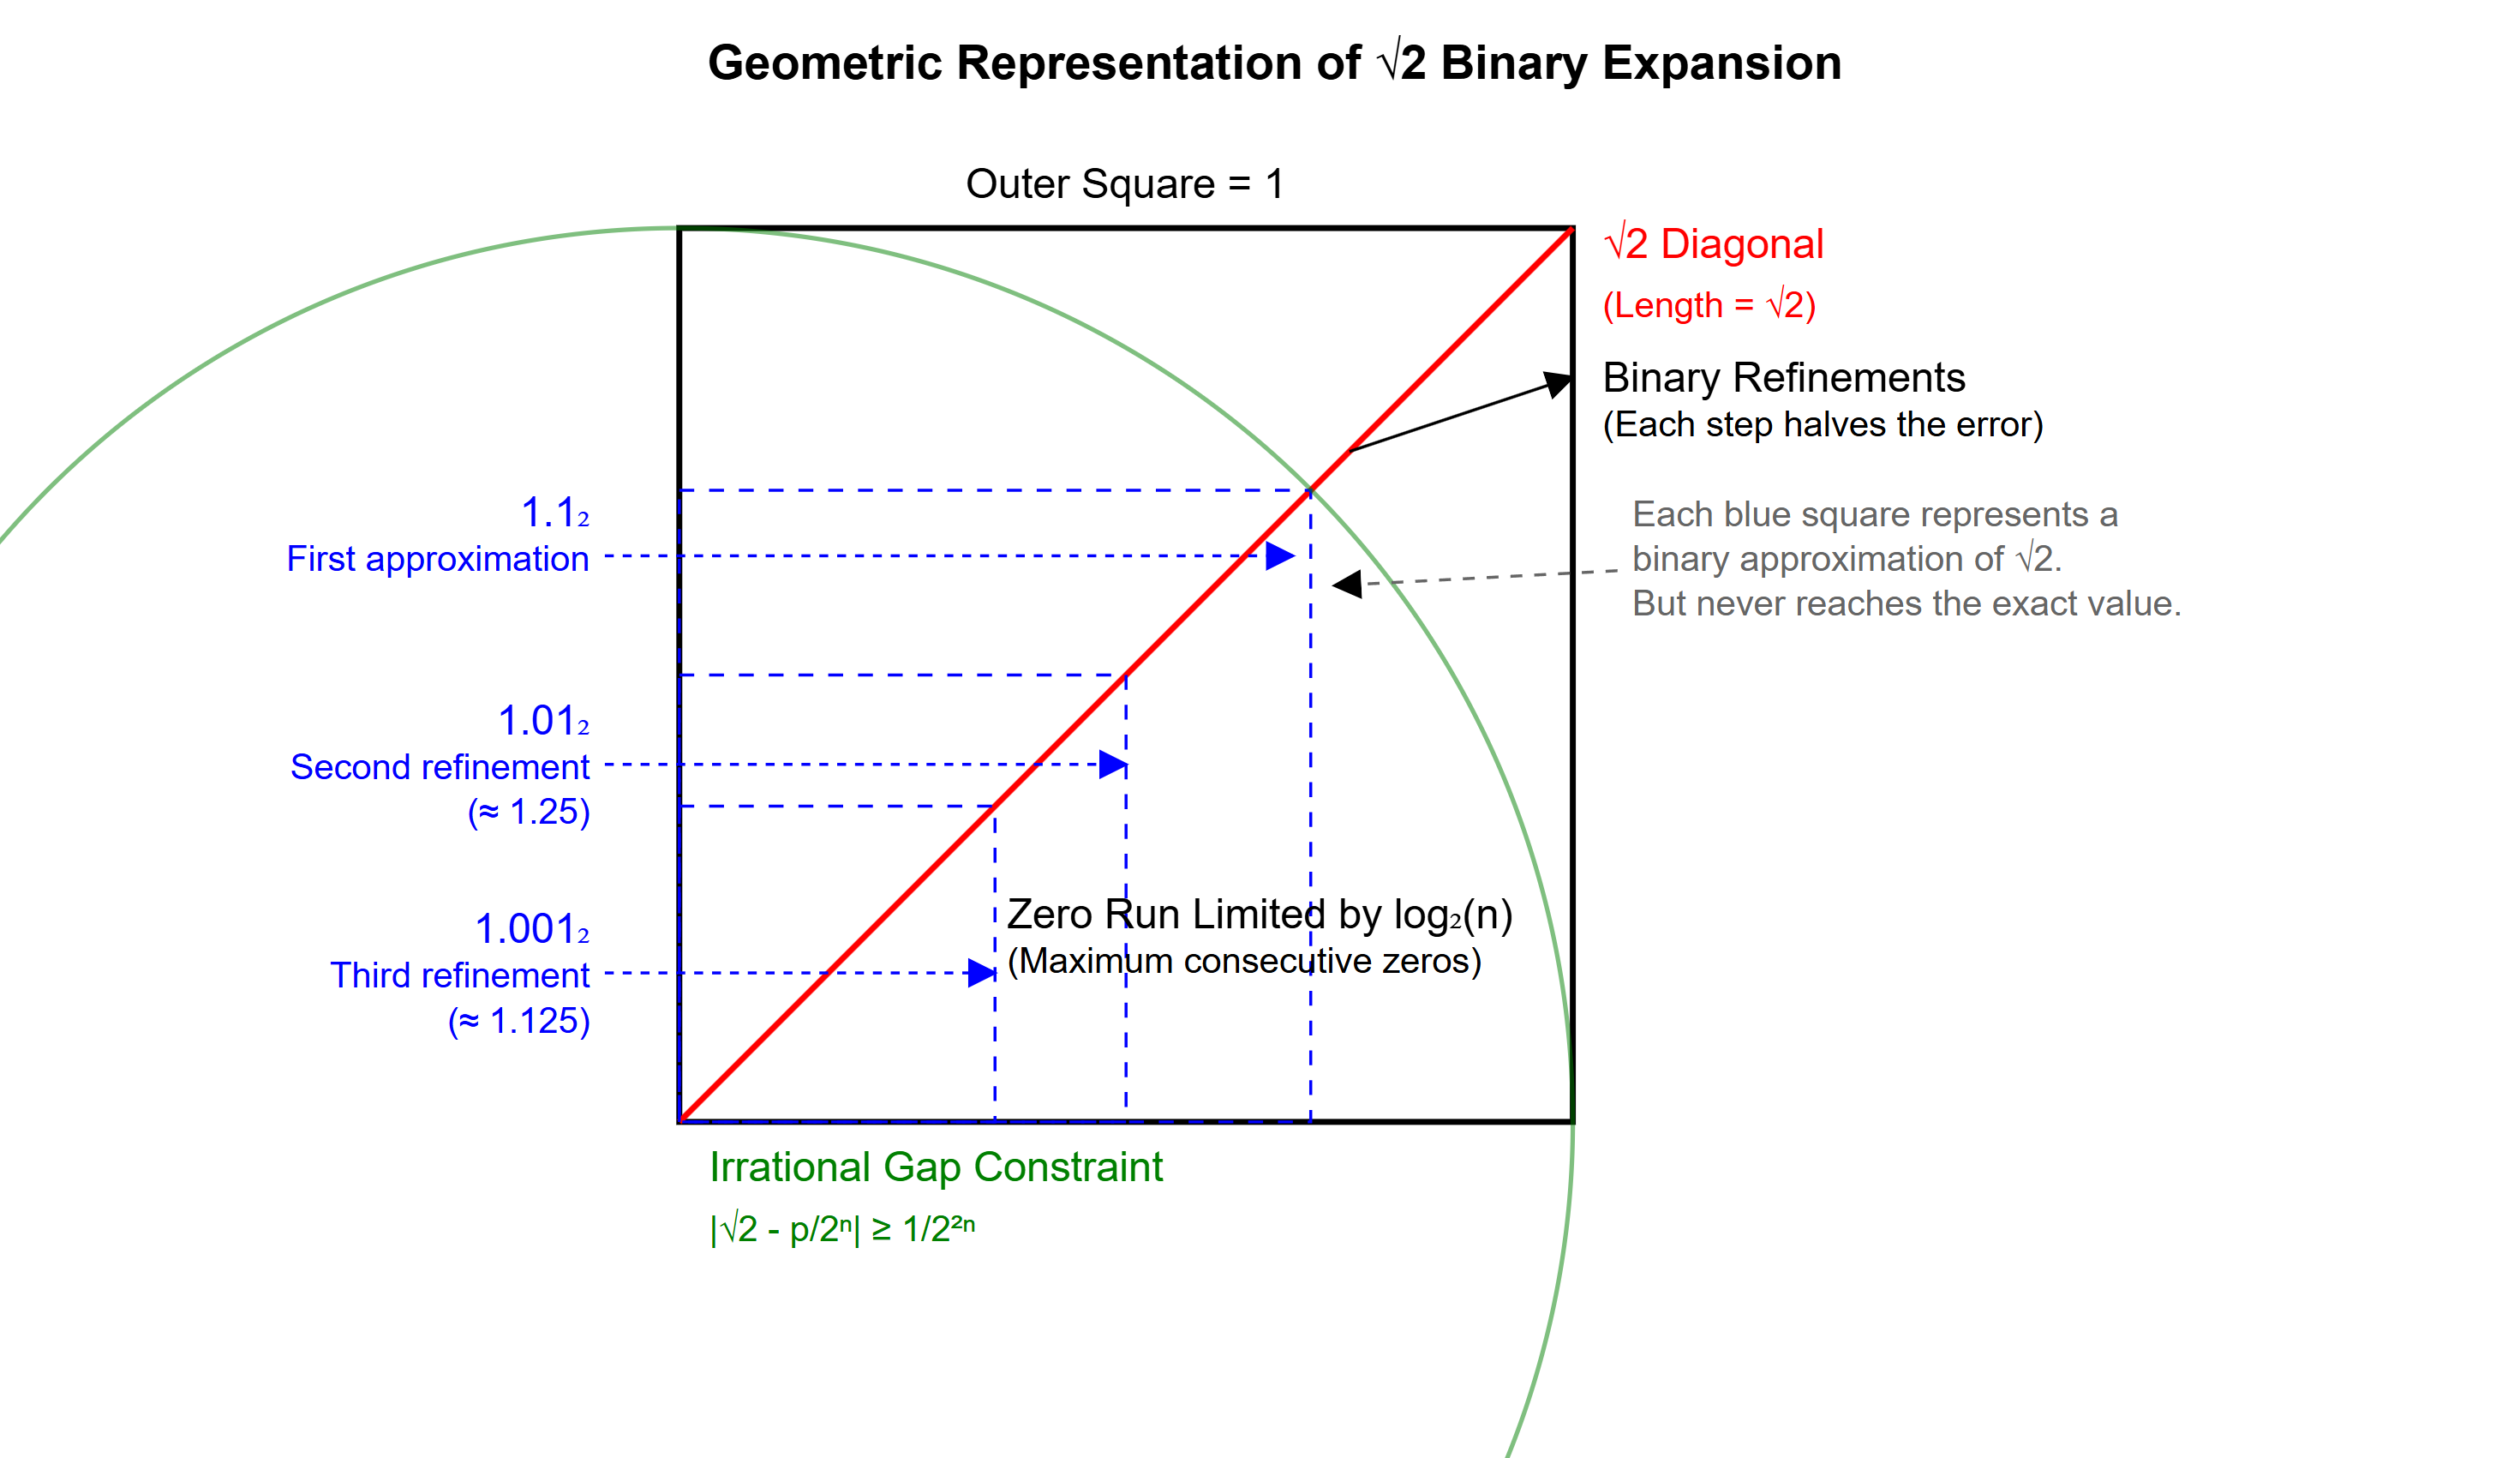
\includegraphics[width=0.8\textwidth]{geometric_diagram_illustrates.png}
    \captionof{figure}{Geometric Representation of $\sqrt{2}$ Binary Expansion. The diagram illustrates successive approximations, the logarithmic constraint on zero runs, and the irrational gap constraint.}
\end{center}

\subsection{Binary Expansion and Approximation}
Each binary digit halves the uncertainty in approximating $\sqrt{2}$. Geometrically:
\begin{itemize}
    \item A run of $k$ zeros signifies no adjustment is needed for $k$ steps.
    \item This corresponds to an approximation accuracy of:
    $$2^{-k}.$$
    \item For instance:
    \begin{itemize}
        \item At $n=1$, $\sqrt{2}$ is approximated as $1.0_2$, overestimating its value.
        \item The next digits, $1.01_2$, refine the approximation, halving the interval of uncertainty.
    \end{itemize}
\end{itemize}

\subsection{Geometric Constraint on Zero Runs}
The limitation on zero runs arises from the following geometric and numerical constraints:
\begin{itemize}
    \item The gap between $\sqrt{2}$ and a rational approximation $\frac{p}{2^n}$ must satisfy:
    $$\left|\sqrt{2} - \frac{p}{2^n}\right| \geq \frac{1}{2^{2n}}.$$
    \item A long zero run of length $k$ implies precision $2^{-k}$, which conflicts with this gap unless:
    $$k \leq \log_2(n).$$
\end{itemize}
This relationship connects the binary structure of $\sqrt{2}$ to its inherent irrationality.

\subsection{Connecting Zero Runs to the Diagram}
The diagram visually demonstrates the following key elements:
\begin{itemize}
    \item \textbf{Red Diagonal:} Represents the infinite precision required to fully describe $\sqrt{2}$.
    \item \textbf{Blue Squares:} Show successive binary refinements, with each step halving the uncertainty.
    \item \textbf{Green Circle:} Encodes the gap constraint, highlighting the impossibility of achieving a perfect finite binary representation.
\end{itemize}
